\documentclass[10pt]{article}
\usepackage[utf8]{inputenc}
\usepackage[T1]{fontenc}
\usepackage[spanish,es-noquoting,es-tabla]{babel}
\usepackage{lmodern}
\usepackage[a4paper,landscape,margin=1.5cm]{geometry}
\usepackage{longtable,array,booktabs}
\usepackage{graphicx}
\usepackage{enumitem}
\usepackage[hidelinks]{hyperref}

\setlength{\parindent}{0pt}
\setlength{\parskip}{4pt}
\newcolumntype{P}[1]{>{\raggedright\arraybackslash}p{#1}}
\setlist{nosep,leftmargin=*}

\begin{document}

\begin{center}
{\Large\bfseries Fase 3. Diseño de la herramienta}\\[2pt]
Radar Tutor UC -- Ciencia de Datos, Unidad 2 -- Universidad de Cuenca
\end{center}

Diseñamos cuatro pantallas: tres para el tutor académico, que es quien toma la decisión, y una para el estudiante. En cada wireframe los números en rojo señalan qué indicador del diccionario de datos (I1 a I7) muestra ese elemento; el detalle está en la tabla que acompaña a cada pantalla. Los wireframes son de baja fidelidad: buscan mostrar qué información aparece y qué acciones se pueden hacer, no el diseño visual final. En la sección 4 del notebook de la prueba de concepto construimos estas mismas cuatro pantallas con datos reales del dataset OULAD.

\begin{center}
\begin{tabular}{P{5.5cm} P{4cm} P{11cm}}
\toprule
\textbf{Pantalla} & \textbf{Actor} & \textbf{Para qué sirve}\\
\midrule
P1. Vista del curso & Tutor académico & Saber a quién contactar primero esta semana.\\
P2. Ficha del estudiante & Tutor académico & Entender por qué un estudiante está en alerta y actuar.\\
P3. Registro de intervención & Tutor académico & Dejar registrada la acción y su seguimiento.\\
P4. Mi progreso & Estudiante & Ver su propia actividad y pedir apoyo.\\
\bottomrule
\end{tabular}
\end{center}

\newpage
\section*{P1. Vista del curso (tutor)}
\begin{center}
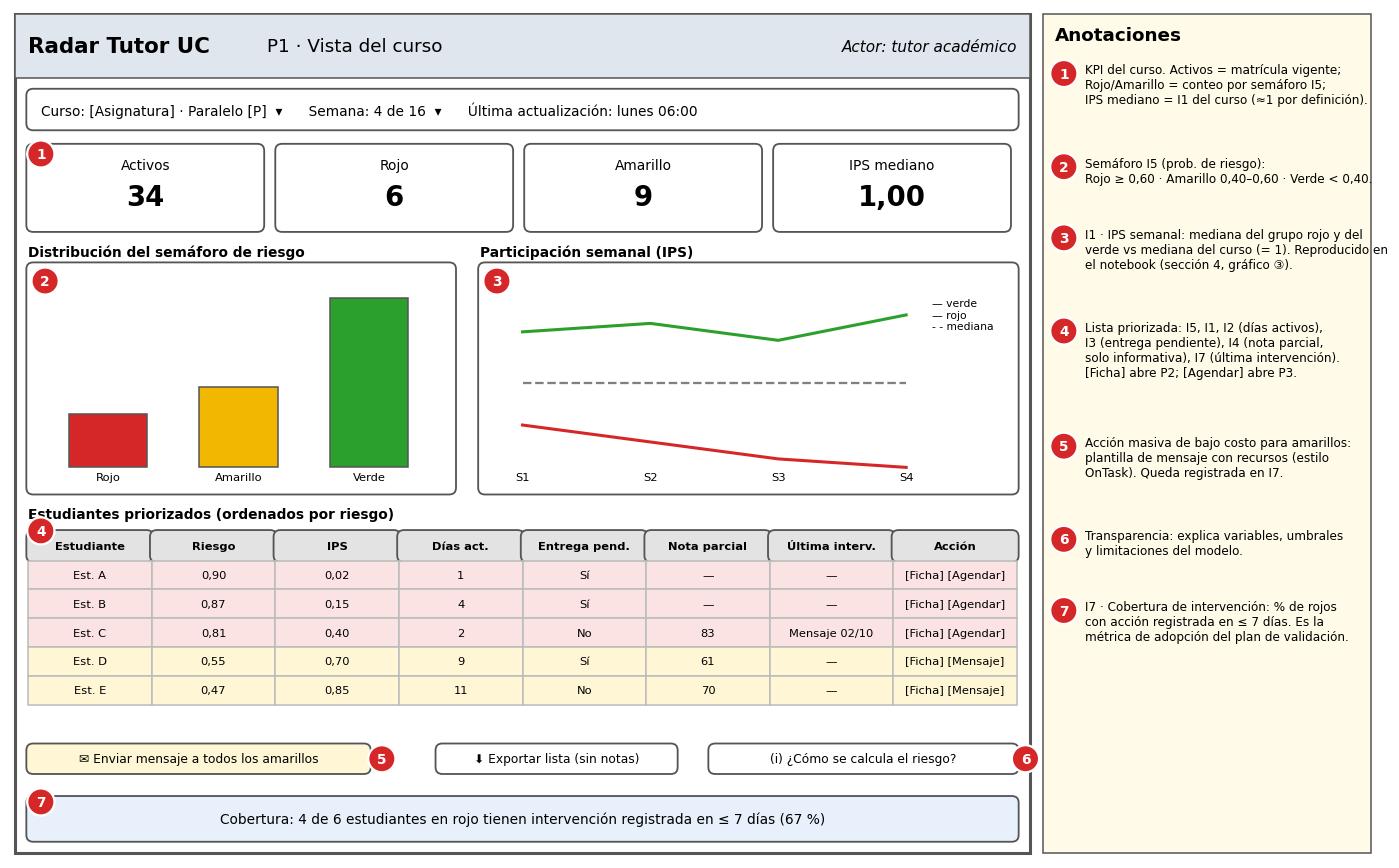
\includegraphics[height=12.2cm]{wireframes/P1_vista_curso.png}
\end{center}
{\small
\begin{tabular}{P{0.8cm} P{8cm} P{15.5cm}}
\toprule
\textbf{N.º} & \textbf{Elemento} & \textbf{Indicador y cálculo}\\
\midrule
1 & Tarjetas: activos, rojos, amarillos, IPS mediano & Conteo por color de I5; mediana de I1 en el curso.\\
2 & Barras del semáforo & I5: rojo desde 0,60; amarillo entre 0,40 y 0,60; verde por debajo de 0,40.\\
3 & Participación semanal & I1 del grupo rojo y del grupo verde frente a la mediana del curso.\\
4 & Lista de estudiantes ordenada por riesgo & I5, I1, I2, I3, I4 y la última intervención (I7). \emph{Ficha} abre P2 y \emph{Agendar} abre P3.\\
5 & Mensaje a todos los amarillos & Envía una plantilla y deja un registro por estudiante (I7).\\
6 & ¿Cómo se calcula el riesgo? & Explica las variables, los umbrales y las limitaciones del modelo.\\
7 & Cobertura & I7: porcentaje de rojos con una acción en 7 días o menos.\\
\bottomrule
\end{tabular}
}

\newpage
\section*{P2. Ficha del estudiante (tutor)}
\begin{center}
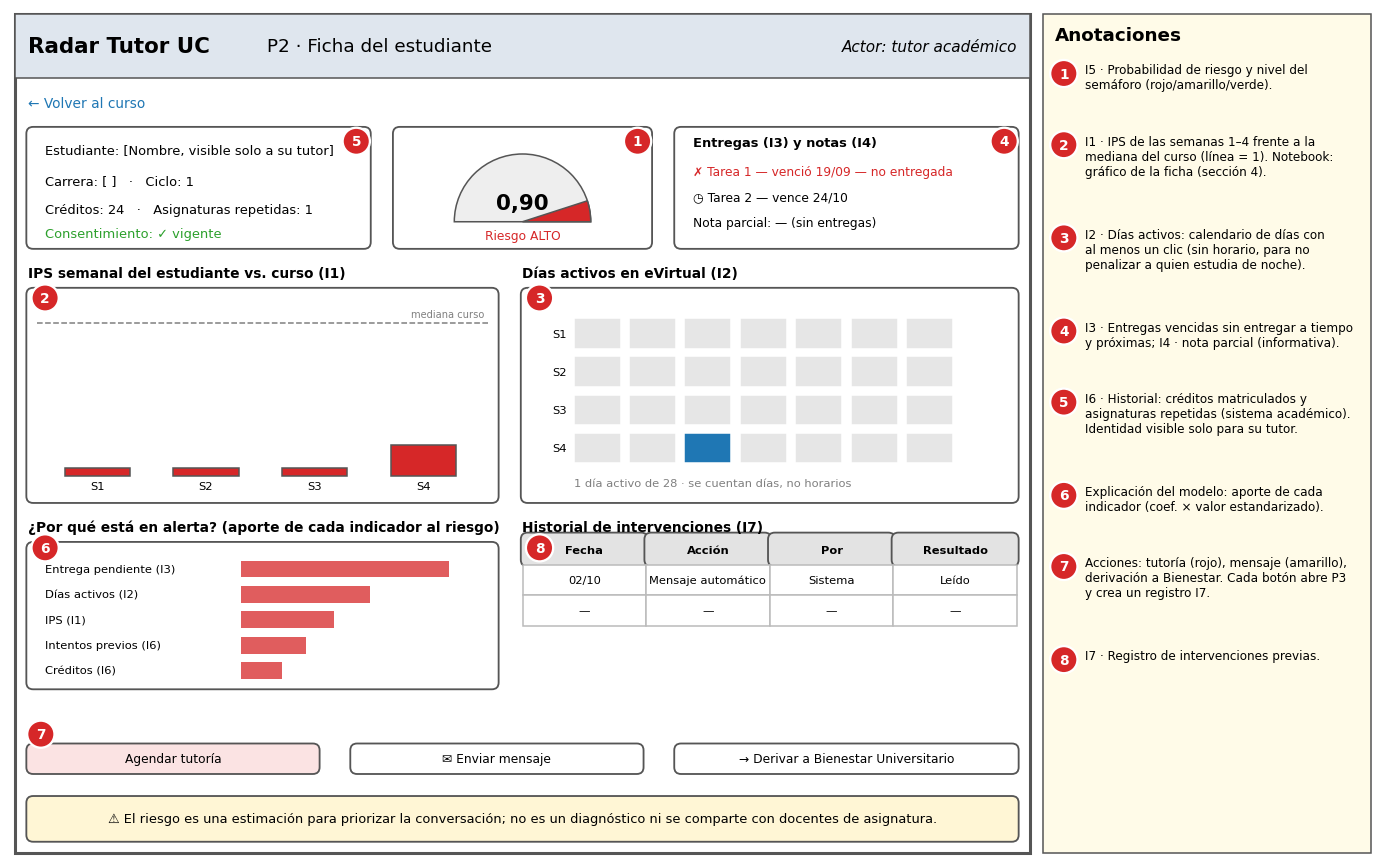
\includegraphics[height=12.2cm]{wireframes/P2_ficha_estudiante.png}
\end{center}
{\small
\begin{tabular}{P{0.8cm} P{11cm} P{12.5cm}}
\toprule
\textbf{N.º} & \textbf{Elemento} & \textbf{Indicador}\\
\midrule
1 & Medidor de riesgo & I5\\
2 & IPS de cada semana frente a la mediana del curso & I1\\
3 & Calendario de días activos & I2\\
4 & Entregas vencidas y próximas, nota parcial & I3 e I4\\
5 & Datos del estudiante: créditos, asignaturas repetidas, consentimiento & I6 y consentimiento\\
6 & ¿Por qué está en alerta? & Aporte de cada variable al modelo de I5\\
7 & Botones: tutoría, mensaje, derivar a Bienestar & Abren P3\\
8 & Historial de intervenciones & I7\\
\bottomrule
\end{tabular}
}

\newpage
\section*{P3. Registro de intervención (tutor)}
\begin{center}
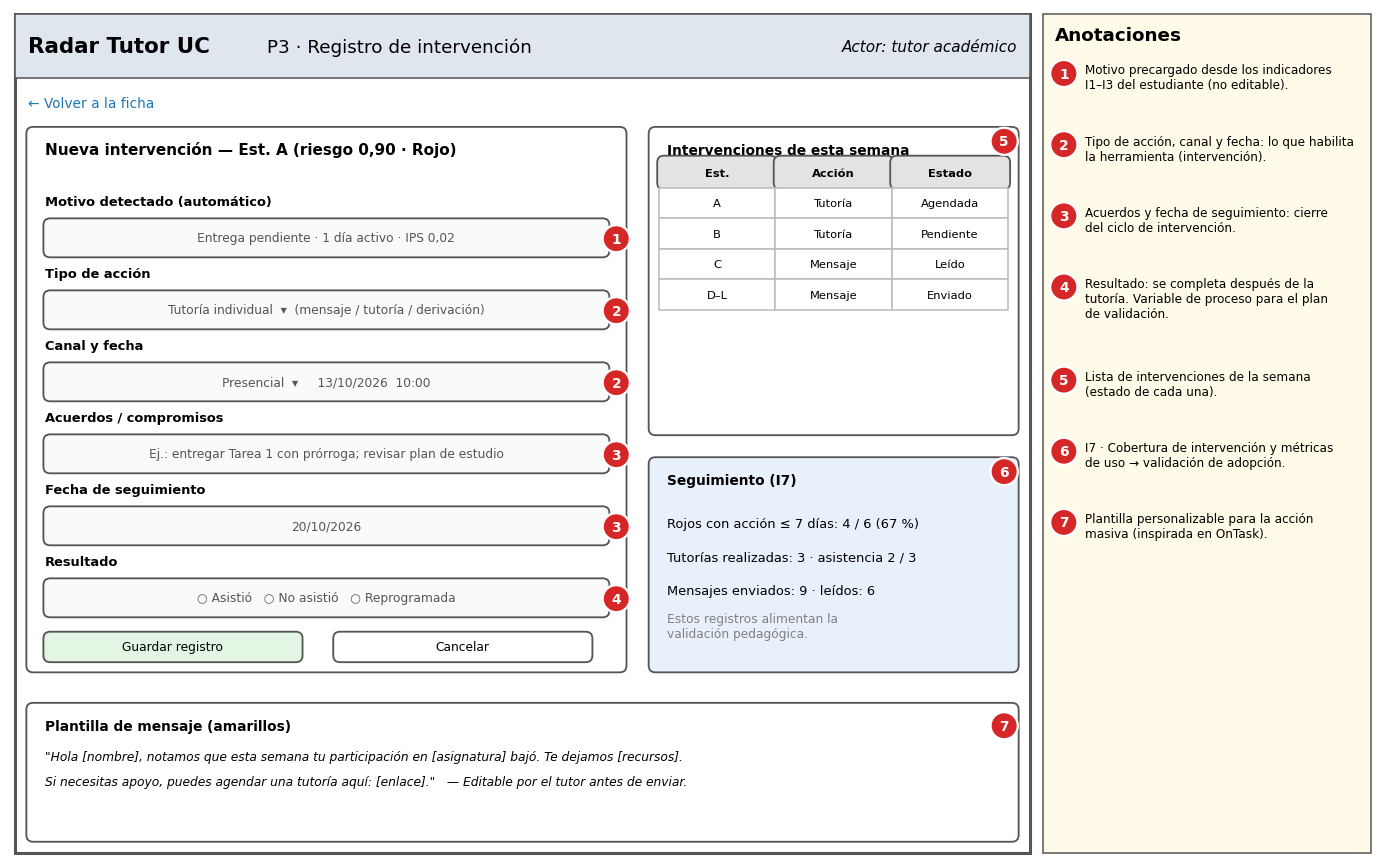
\includegraphics[height=12.2cm]{wireframes/P3_registro_intervencion.png}
\end{center}
{\small
\begin{tabular}{P{0.8cm} P{11cm} P{12.5cm}}
\toprule
\textbf{N.º} & \textbf{Elemento} & \textbf{Indicador o dato}\\
\midrule
1 & Motivo detectado (se completa solo) & I1, I2 e I3 del estudiante\\
2 & Tipo de acción, canal y fecha & Registro de intervención\\
3 & Acuerdos y fecha de seguimiento & Registro de intervención\\
4 & Resultado (asistió, no asistió, reprogramada) & Registro de intervención; se usa en el plan de validación\\
5 & Intervenciones de la semana & Registro de intervención\\
6 & Seguimiento & I7\\
7 & Plantilla de mensaje & --\\
\bottomrule
\end{tabular}
}

\newpage
\section*{P4. Mi progreso (estudiante)}
\begin{center}
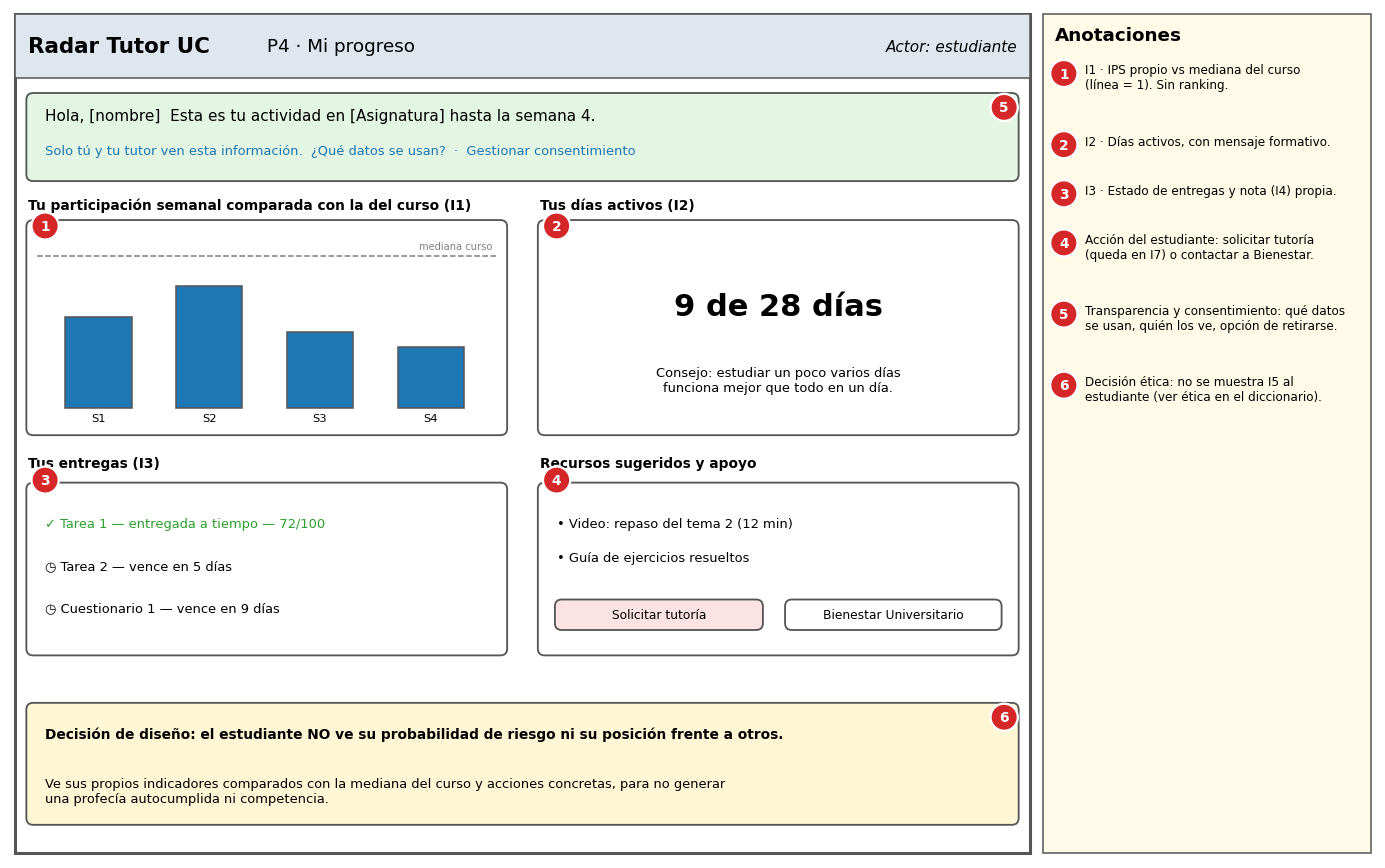
\includegraphics[height=12.2cm]{wireframes/P4_mi_progreso_estudiante.png}
\end{center}
{\small
\begin{tabular}{P{0.8cm} P{11cm} P{12.5cm}}
\toprule
\textbf{N.º} & \textbf{Elemento} & \textbf{Indicador}\\
\midrule
1 & Participación semanal propia frente a la mediana, sin ranking & I1\\
2 & Días activos, con un consejo & I2\\
3 & Entregas y nota propia & I3 e I4\\
4 & Recursos y botón para pedir tutoría & Queda en el registro de intervenciones\\
5 & Qué datos se usan y opción de retirar el consentimiento & Consentimiento\\
6 & El estudiante no ve su probabilidad de riesgo & Decisión ética (ver diccionario de datos, sección de ética)\\
\bottomrule
\end{tabular}
}

\newpage
\section*{Flujo de intervención}
\begin{center}
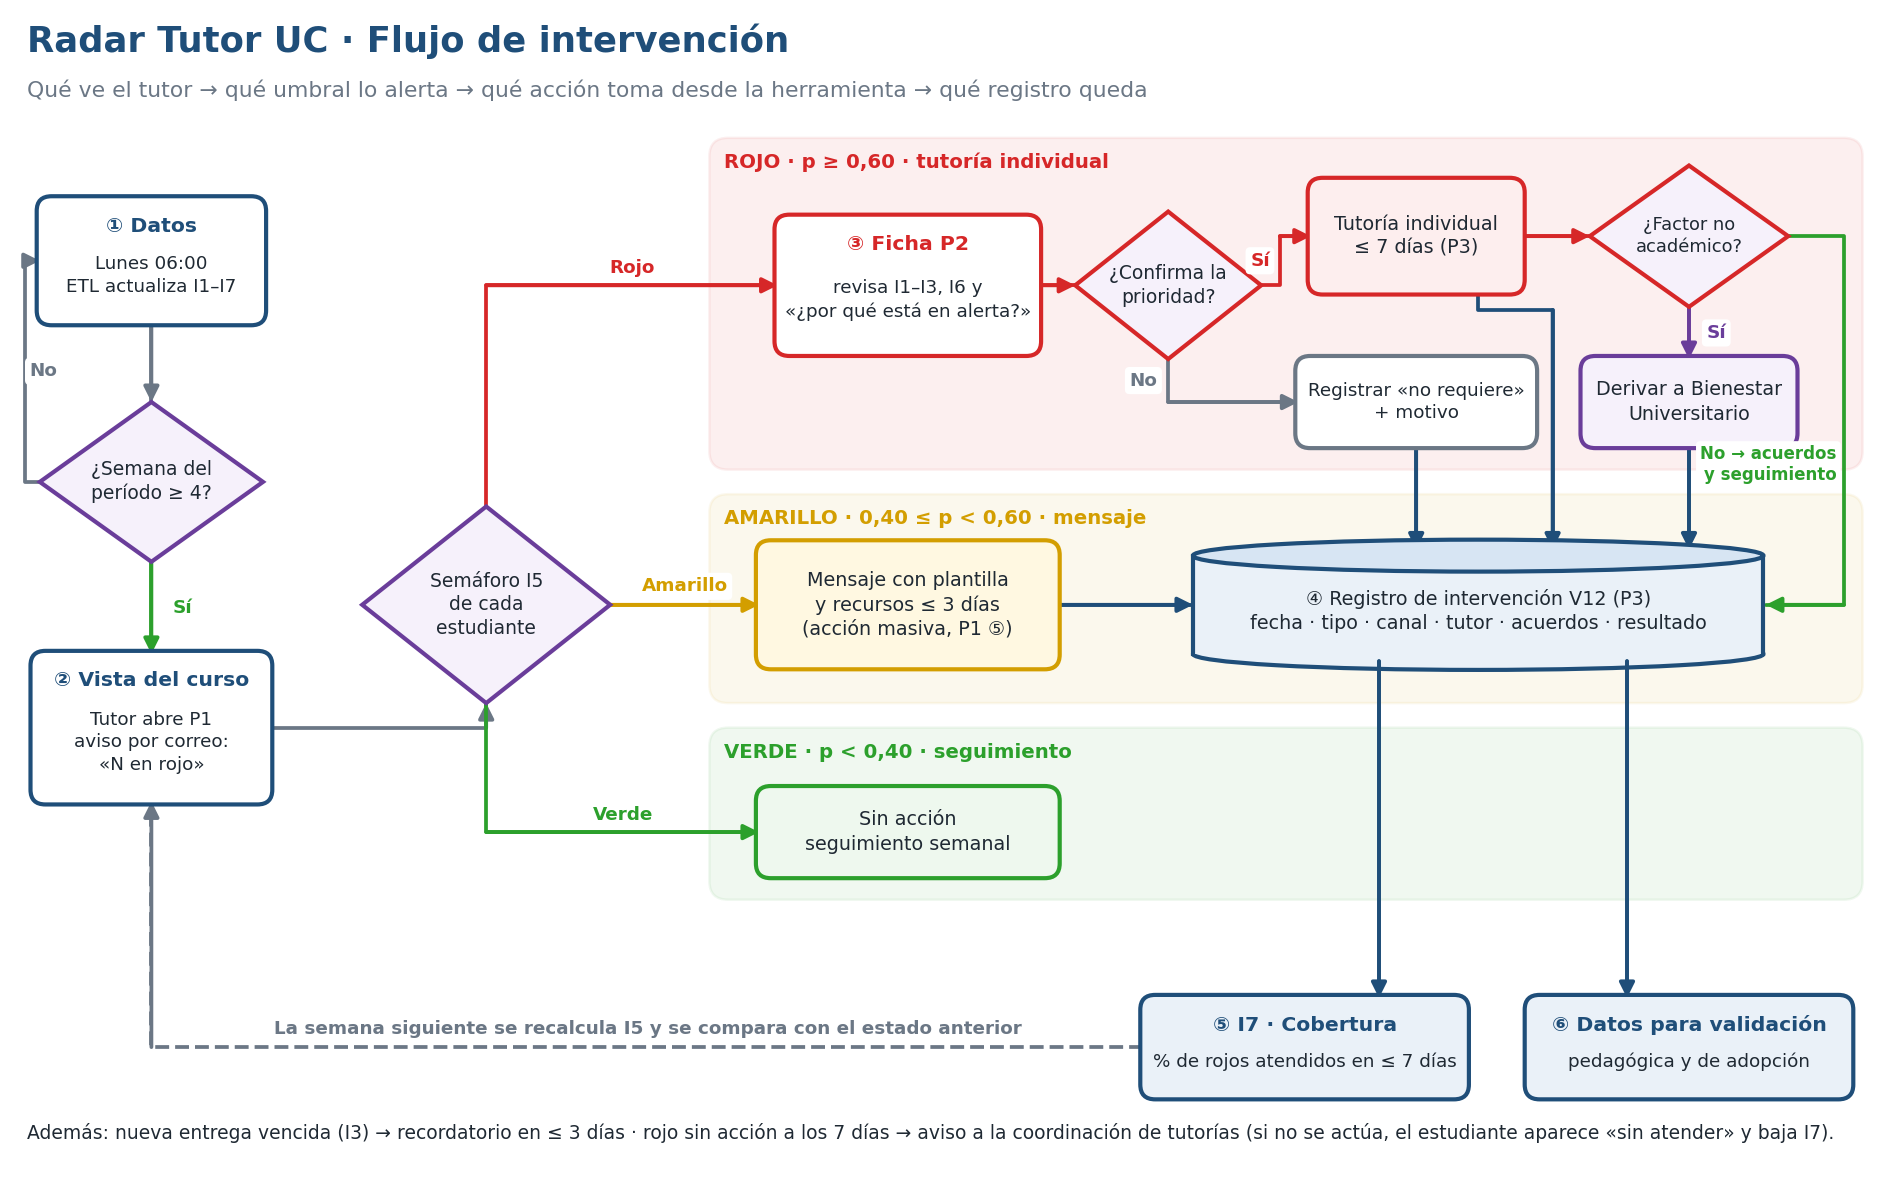
\includegraphics[height=11.6cm]{flujo_intervencion.png}
\end{center}
{\small
\begin{tabular}{P{3.8cm} P{3.2cm} P{3.3cm} P{5.5cm} P{1.6cm} P{6.4cm}}
\toprule
\textbf{Señal} & \textbf{Umbral} & \textbf{Quién actúa} & \textbf{Acción} & \textbf{Plazo} & \textbf{Qué queda registrado}\\
\midrule
Rojo (I5) & 0,60 o más & Tutor & Tutoría individual & 7 días & Intervención de tipo tutoría\\
Amarillo (I5) & Entre 0,40 y 0,60 & Tutor (envío masivo) & Mensaje con recursos e invitación a tutoría & 3 días & Intervención de tipo mensaje\\
Nueva entrega vencida (I3) & Una evaluación no entregada & Tutor & Recordatorio & 3 días & Intervención de tipo recordatorio\\
Rojo sin atender & 7 días sin registro & Sistema & Aviso al tutor y a la coordinación de tutorías & -- & Baja la cobertura I7\\
Problema no académico & Criterio del tutor & Bienestar Universitario & Derivación & -- & Intervención de tipo derivación\\
\bottomrule
\end{tabular}
}

\textbf{¿Y si nadie actúa?} El estudiante sigue en rojo la semana siguiente y aparece como \emph{sin atender}. La coordinación de tutorías puede ver la cobertura de cada tutor. En la validación, este registro nos permite separar dos situaciones muy distintas: que la herramienta no funcione o que simplemente no se haya usado.

\newpage
\section*{Arquitectura de alto nivel}
\begin{center}
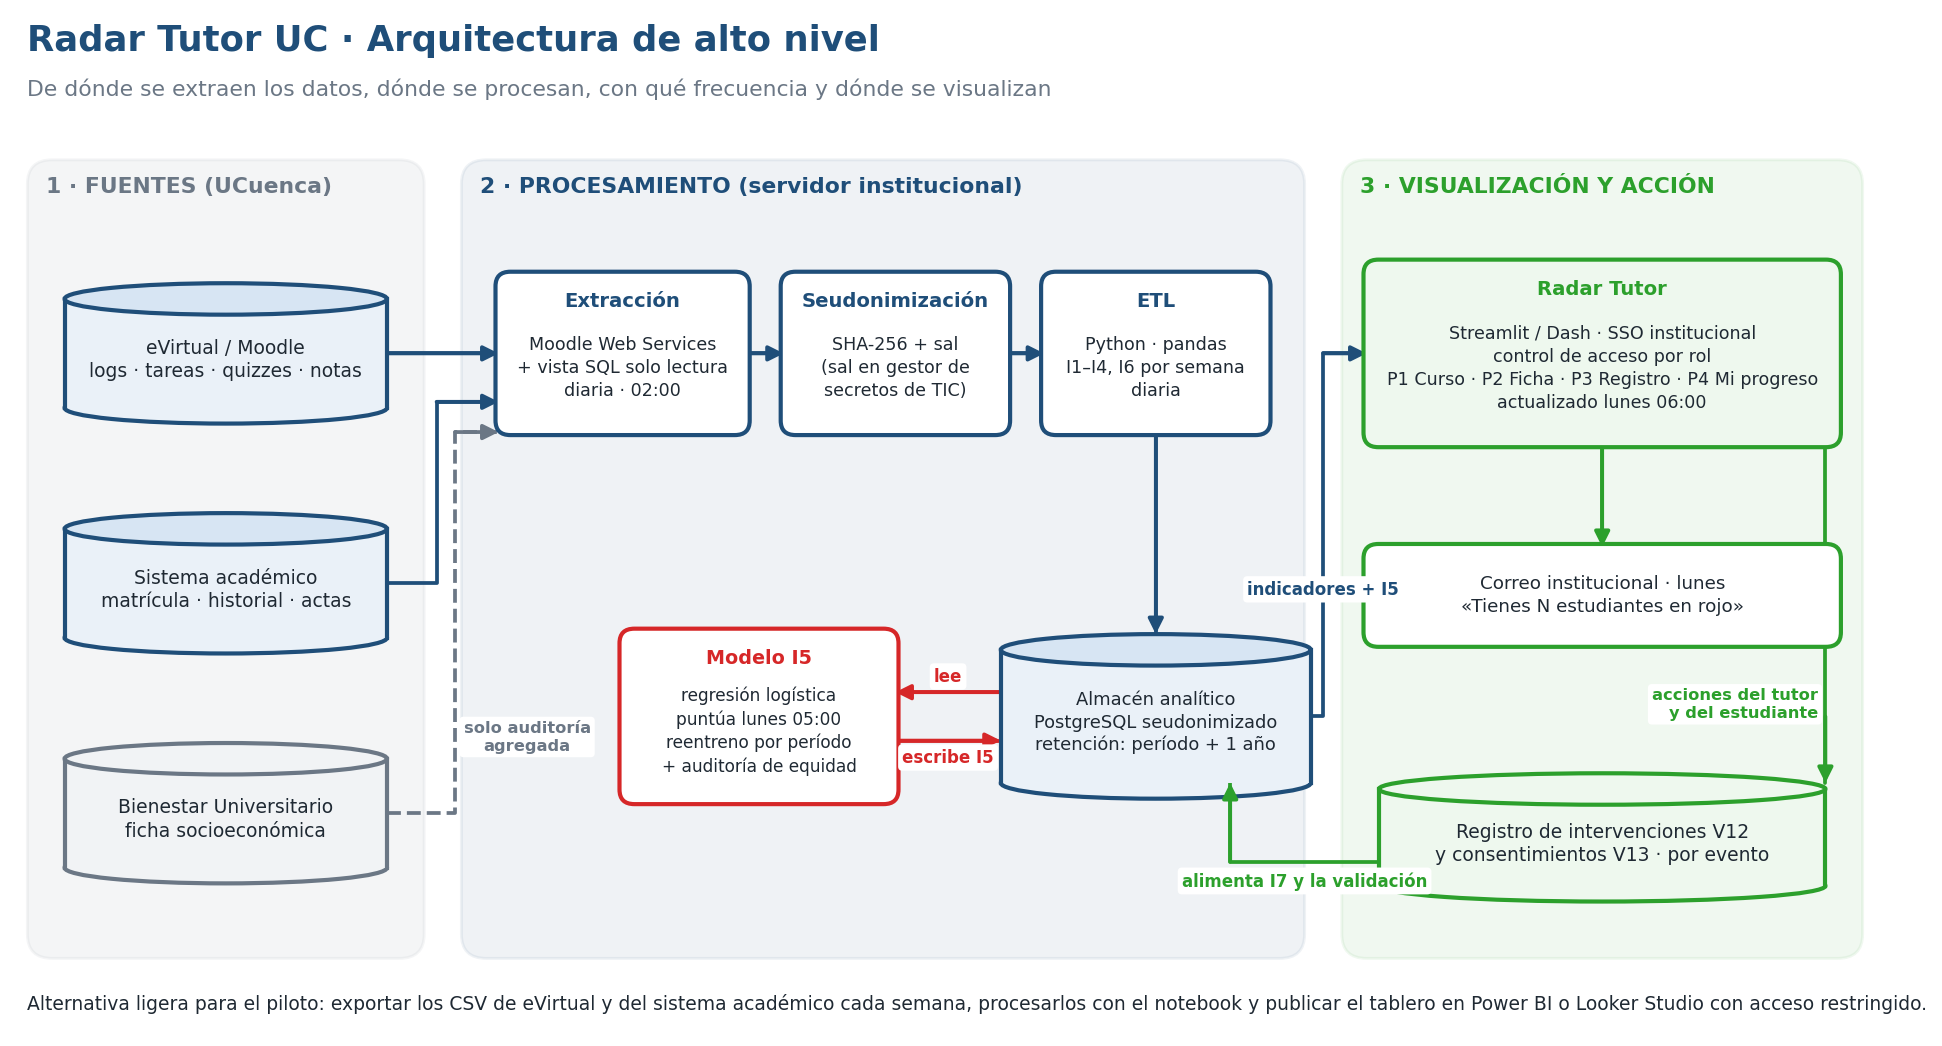
\includegraphics[height=10.4cm]{arquitectura.png}
\end{center}
{\small
\begin{tabular}{P{3.5cm} P{13.5cm} P{7cm}}
\toprule
\textbf{Etapa} & \textbf{Cómo} & \textbf{Frecuencia}\\
\midrule
Extracción & Servicios web de Moodle (eVirtual) y una consulta de solo lectura al sistema académico. & Diaria (02:00) para la actividad; por período para la matrícula y el historial.\\
Seudonimización & Script en Python con una clave que custodia la Dirección de TIC. & En cada extracción.\\
Procesamiento & Python y pandas, con el mismo código del notebook de la prueba de concepto. & Diario.\\
Modelo I5 & Regresión logística con scikit-learn. & Cálculo cada lunes a las 05:00; reentrenamiento cada período.\\
Almacenamiento & Base de datos PostgreSQL en un servidor de la universidad. & Continuo.\\
Visualización & Aplicación en Streamlit o Dash con el usuario institucional y permisos por rol. & Actualización los lunes a las 06:00.\\
Avisos y registro & Correo institucional; tablas de intervenciones y consentimientos en la misma base de datos. & Avisos los lunes; registro en cada acción.\\
\bottomrule
\end{tabular}
}

Para un primer piloto sin integración con TIC bastaría con exportar cada semana los archivos CSV de eVirtual y del sistema académico, procesarlos con el notebook y publicar el tablero en Power BI o Looker Studio con acceso restringido. Como aprendieron los equipos del proyecto LALA, empezar con los datos que la universidad ya tiene facilita mucho el pilotaje.

\end{document}
